\chapter{Approach}
\label{cha:Approach}
In the last section a few approaches have been outlined and discussed, that have successfully implemented methods regarding the creation of audios/music with a neural network approach. As seen, these have been mainly categorized in neural audio synthesis and neural audio style transfer. There current work has its main influence from the area neural audio synthesis, and can be categorized as such, as the methodology and workflow is strongly related to those works. Nevertheless regarding certain components, it has also its influence from the style transfer methods, despite not defining a specific content or style audio respective loss functions.

This chapter will therefore dive into the methodology and exact workflow of this works' solution, to the problem that also will help to derive the answers to the defined research questions. First an Overview/Motivation should provide the reader with the intended idea and an overview of the applied methods, to get a general understanding of the idea (see section \ref{sec:app_motivation}. Later on the single steps and components that are needed, in order reach the desired functionalities, are going to get described in detail, starting with the pre processing. Further on the ML-Model (neural network) will get described, as well as the step that is done to synthesize new sounds. Further on, the required steps for (re)generating a listenable audio as well as an description of the used dataset for training and also all experiments conducted later on (see chapter \ref{cha:Experiment}).

\section{Motivation}
\label{sec:app_motivation}
Like mentioned in the beginning of this thesis, this work aims to explore the possibilities of machine learning techniques such as neural networks, to apply in the audio domain for sound generation. This idea is mainly inspired by the idea of taking two distinct audio sources and mixing their characteristics in order to generate a new sound. As seen in the previous chapter, this idea is strongly related to the image domain, where the "synthesis" of a new pictures based on two source images, is commonly known as image style transfer (point \ref{sec:rw_imgstyletransfer}). This technique, of having a content image to be stylised with a certain style from another image, would mean for the application in the audio, to have a style sound to be transferred onto a content/target sound. Such approaches are specifically known as audio style transfer and can either be applied to single notes or also whole audio samples or songs. Having the principle of content and style this would mean, that of one sound the global structure and rhythmical components get preserved while imposing style (e.g. the timbre) on it to generate audios. The details to these approaches, have already been outlined in the previous chapter, when describing some existing work around this topic.

Neural audio synthesis is another method for neural sound generation, which does not apply the principles of style and content audio. In the previous chapter, some insights could be gained, how neural audio synthesis can look like, as well as how it can be achieved using different methods and neural networks. Most of those methods, were showing promising results, either concerning the auditory quality but also the possibilities that arise in experimenting and designing sounds. Those methods were using most of the time so called autoencoder networks, that can be used for dimensionality reduction of input data, as they have a so called "bottleneck" in the middle. \cite{hinton2006autoencoder} Because of this structure, the compressed data in this "bottleneck" represents essential features that either can be combined/interpolated or directly synthesized. To generate synthesized audio, the solutions described in section \ref{sec:rw_neural_audio_synthesis} used the "decompressing part" of the network to generate in order audio data. The exact workflow and methodologies for sound creation, have already been mentioned in the chapter related works (see chapter \ref{cha:related_works}, point \ref{sec:rw_neural_audio_synthesis}).

Out of those methodologies, when having the idea of using two instruments' characteristics, to generate audio, the approach of \textit{Engel et al.} \cite{Engel2017} using convolutional and WaveNet-style autoencoders yielded the most promising results. Promising especially in terms of output quality but also concerning its implementation/reproducability. With a provided interactive web application, the results of this solutions can be explored, whereas different sounds can be mixed based with a certain ratio. The results in the web application are based on the WaveNet-style autoencoder but according to the scientific article, the convolutional (baseline) also provides strong results. Implementing an approach with a WaveNet-style network would also go beyond the scope, not least also the computational costs would be too high. As also some audio style transfer methods, especially the approach by \textit{Ramani et al.} \cite{Ramani2018}, are using convolutional autoencoders, this kind of network was chosen to be preferable, to be applied in this work/research.

\section{Overview}
\label{sec:app_overview}
Based on the motivation and existing approaches, this work aims to propose a system, that uses a convolutional autoencoder network, for the task of neural audio synthesis. This systems' goal is to take two distinct audio samples as input, wheras the significant features, of those get extracted and interpolated, to in order (re)generate a novel sound in the end. In figure \ref{fig:toolchain} the general workflow of the toolchain is depicted in order to get an understanding, how this system is built up. 

 \begin{figure}[htb!]
	\caption{Overview of the proposed solution}
	\label{fig:toolchain}
	\centering
	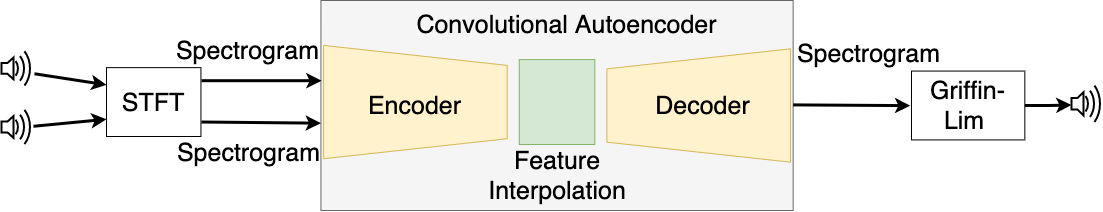
\includegraphics[width=\textwidth]{images/approach/Toolchain.png}
\end{figure}

Starting on the very left, two audios are taken and have to be brought into a suitable representation for this type of network. As audio is in its raw form a time-continuous signal and the input for convolutional networks are of a different shape (e.g. images) some pre-processing has to be done. In this case the short-term Fourier transform (STFT) is applied in order to generate a spectrogram, that shows the frequency spectra over the time. The frequency spectra contains on the one hand the magnitude (power) of the frequencies but also the phase information. For this purpose, only the magnitude data gets used, as its found to contain the most characteristic features of an audio. The ML-model (autoencoder) then takes the magnitude data as input, from which a compressed representation with the essential features gets generated with the lefthand (encoder) side. Having those features of two different audio samples, those get linearly interpolated, to generate one feature vector representing the "mixed" features of two instruments. This new vector, gets passed through the righthand (decoder) side of the network, which regenerates again spectral magnitude data of the same dimension as the input. In order to obtain a "playable" audio sound, it gets transformed back into time-domain with the Griffin-Lim algorithm \cite{Griffin1984} for phase estimation or the inverse short-term Fourier transform (ISTFT). The latter will be applied if there was no interpolation in the embedded space, as the phase information can be reused. Corresponding terminologies as well as a detailed insight into each step and its functionalities are given down below in the following points.

\section{Pre Processing}
\label{sec:app_pre-processing}
Pre-processing is the task of preparing raw data for a specific purpose


\subsection{Spectrograms and STFT}



\section{ML-Model}
\label{sec:app_model}

\section{Post Processing}
\label{sec:app_sec_post_processing}

\section{Interpolation in latent space}
\label{sec:app_interpolation}

\section{Dataset}
\label{sec:app_dataset}